\documentclass[tikz,border=10pt]{standalone}
\usepackage{helvet}
\renewcommand{\familydefault}{\sfdefault}
\usepackage{tikz}
\usepackage{tikz-3dplot}
\usetikzlibrary{shapes, arrows.meta, positioning, calc, fit, decorations.pathreplacing, 3d}

\definecolor{emeraldpine}{HTML}{1A4D3E}
\definecolor{harvardcrimson}{HTML}{A51C30}
\definecolor{ethdarkblue}{HTML}{1F407A}
\definecolor{ethpetrol}{HTML}{007A87}
\definecolor{ethbronze}{HTML}{B87333}
\definecolor{ethpurple}{HTML}{5B4B8A}
\definecolor{ink}{HTML}{1A202C}
\definecolor{softink}{HTML}{4A5568}
\definecolor{paleink}{HTML}{A0AEC0}
\definecolor{cardbg}{HTML}{F8FAFC}
\definecolor{shadecolor}{HTML}{F4F6F9}

\begin{document}
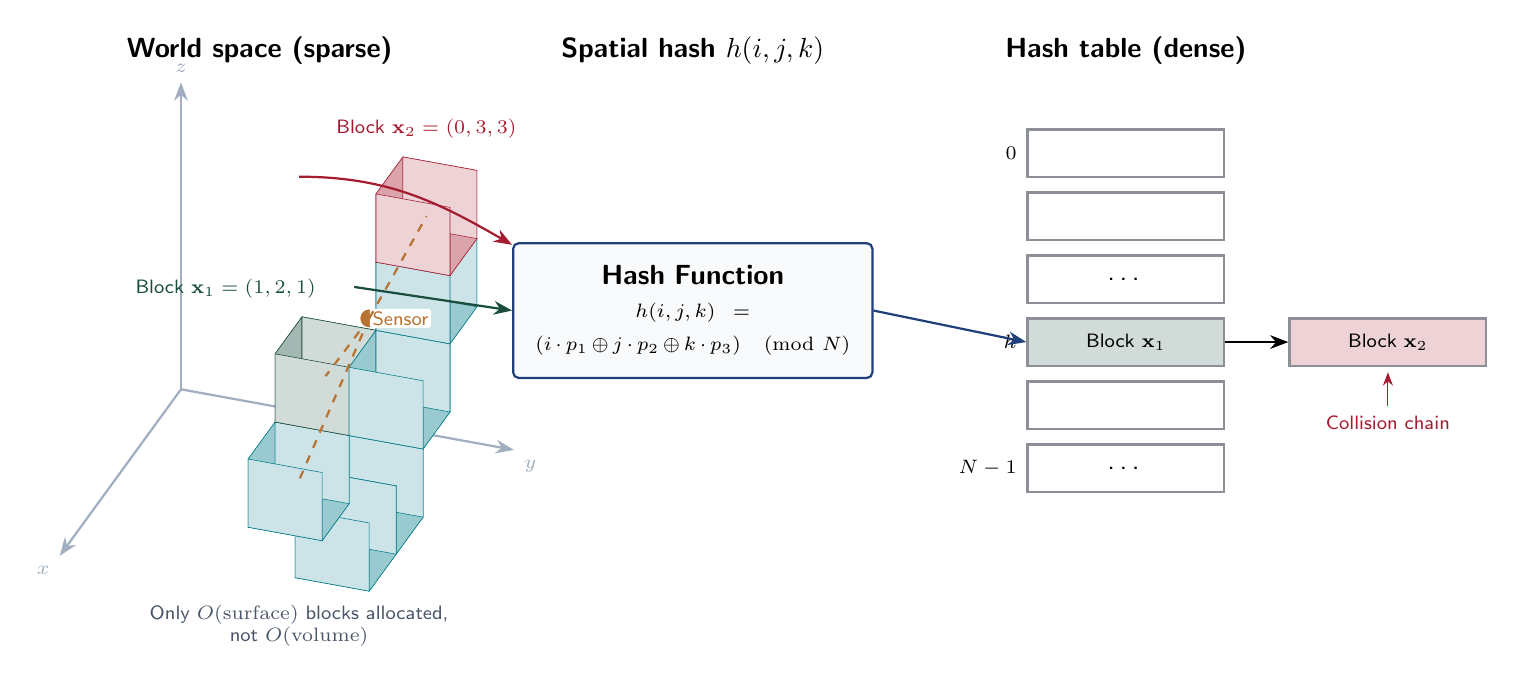
\begin{tikzpicture}[
    font=\sffamily,
    >=Stealth,
    block/.style={draw=ethdarkblue, fill=cardbg, thick, rounded corners=2pt, align=center},
    bucket/.style={draw=ink!50, fill=white, thick, minimum width=2.5cm, minimum height=0.6cm},
    ptr/.style={draw=ethdarkblue, fill=ethdarkblue, circle, inner sep=1.5pt}
]

% Panel 1: World Space (3D)
\node[anchor=south, font=\bfseries] at (1, 4.5) {World space (sparse)};

\tdplotsetmaincoords{60}{110}
\begin{scope}[shift={(0,0.5)}, tdplot_main_coords]
    % Draw some axes
    \draw[->, thick, paleink] (0,0,0) -- (4.5,0,0) node[anchor=north east]{\scriptsize $x$};
    \draw[->, thick, paleink] (0,0,0) -- (0,4.5,0) node[anchor=north west]{\scriptsize $y$};
    \draw[->, thick, paleink] (0,0,0) -- (0,0,4.5) node[anchor=south]{\scriptsize $z$};

    % Define a macro to draw a voxel block
    \def\drawblock#1#2#3#4{
        \begin{scope}[shift={(#1,#2,#3)}]
            \draw[fill=#4!80!white, draw=#4, very thin] (0,0,0) -- (1,0,0) -- (1,1,0) -- (0,1,0) -- cycle;
            \draw[fill=#4!60!white, draw=#4, very thin] (0,0,1) -- (1,0,1) -- (1,1,1) -- (0,1,1) -- cycle;
            \draw[fill=#4!40!white, draw=#4, very thin] (0,0,0) -- (0,0,1) -- (1,0,1) -- (1,0,0) -- cycle;
            \draw[fill=#4!40!white, draw=#4, very thin] (0,1,0) -- (0,1,1) -- (1,1,1) -- (1,1,0) -- cycle;
            \draw[fill=#4!20!white, draw=#4, very thin] (0,0,0) -- (0,0,1) -- (0,1,1) -- (0,1,0) -- cycle;
            \draw[fill=#4!20!white, draw=#4, very thin] (1,0,0) -- (1,0,1) -- (1,1,1) -- (1,1,0) -- cycle;
        \end{scope}
    }

    % Surface curve representation - sorted back to front (rough estimate based on angles)
    % Angle 110: y goes "back/left", x goes "forward/left", z goes "up"
    \drawblock{2}{3}{0}{ethpetrol}
    \drawblock{3}{3}{0}{ethpetrol}
    \drawblock{2}{2}{0}{ethpetrol}
    \drawblock{1}{2}{1}{emeraldpine} % Selected block
    \drawblock{1}{3}{1}{ethpetrol}
    \drawblock{0}{3}{2}{ethpetrol}
    \drawblock{0}{3}{3}{harvardcrimson} % Colliding block
    
    % Robot / Sensor origin
    \filldraw[ethbronze] (4, 4, 4) circle (3pt) node[anchor=west, font=\scriptsize, fill=white, inner sep=1pt, rounded corners=1pt]{Sensor};
    \draw[dashed, ethbronze, thick] (4,4,4) -- (1.5, 2.5, 1.5);
    \draw[dashed, ethbronze, thick] (4,4,4) -- (2.5, 2.5, 0.5);
    \draw[dashed, ethbronze, thick] (4,4,4) -- (0.5, 3.5, 3.5);
    
    % Annotations
    \node[anchor=south east, font=\scriptsize, text=emeraldpine] at (1.5, 2.5, 2.5) {Block $\mathbf{x}_1=(1,2,1)$};
    \node[anchor=south, font=\scriptsize, text=harvardcrimson] at (0.5, 3.5, 4.5) {Block $\mathbf{x}_2=(0,3,3)$};
\end{scope}

\node[font=\scriptsize\color{softink}, align=center] at (1.5, -2.5) {Only $O(\mathrm{surface})$ blocks allocated,\\not $O(\mathrm{volume})$};

% Middle Panel: Hash Function
\node[anchor=south, font=\bfseries] at (6.5, 4.5) {Spatial hash $h(i,j,k)$};

\node[block, text width=4cm, inner sep=8pt] (hashfunc) at (6.5, 1.5) {
    \textbf{Hash Function}\\
    \vspace{4pt}
    \scriptsize
    $h(i,j,k) = $\\
    $(i \cdot p_1 \oplus j \cdot p_2 \oplus k \cdot p_3) \pmod N$
};

\draw[->, thick, emeraldpine] (2.2, 1.8) -- (hashfunc.west);
\draw[->, thick, harvardcrimson] (1.5, 3.2) to[out=0, in=150] (hashfunc.160);

% Right Panel: Hash Table
\node[anchor=south, font=\bfseries] at (12, 4.5) {Hash table (dense)};

\begin{scope}[shift={(12, -0.5)}]
    % Draw Hash Table
    \foreach \i/\text in {0/\dots, 1/ , 2/ , 3/\dots, 4/ , 5/ } {
        \node[bucket] (bucket\i) at (0, \i*0.8) {\text};
    }
    \node[anchor=east, font=\scriptsize] at (bucket0.west) {$N-1$};
    \node[anchor=east, font=\scriptsize] at (bucket5.west) {$0$};
    
    % Bucket 2 has our entries
    \node[bucket, fill=emeraldpine!20] (bucket2) at (0, 2*0.8) {\scriptsize Block $\mathbf{x}_1$};
    \node[anchor=east, font=\scriptsize] at (bucket2.west) {$h$};
    
    % Collision chain
    \node[bucket, fill=harvardcrimson!20, right=0.8cm of bucket2] (chain1) {\scriptsize Block $\mathbf{x}_2$};
    
    % Pointers
    \draw[->, thick] (bucket2.east) -- (chain1.west);
    
    \node[below=0.5cm of chain1, text width=2cm, align=center, font=\scriptsize\color{harvardcrimson}] (coltext) {Collision chain};
    \draw[->, harvardcrimson, shorten >=2pt] (coltext) -- (chain1);
\end{scope}

\draw[->, thick, ethdarkblue] (hashfunc.east) -- (bucket2.west);

\end{tikzpicture}
\end{document}
